%======================================================================
\chapter{Lab Setup}
%======================================================================

%----------------------------------------------------------------------
\section{USB}
%----------------------------------------------------------------------


%----------------------------------------------------------------------
\section{Raspberry Pi}
%----------------------------------------------------------------------
The communication protocol utilized by the Q-Flex2 embedded panel is SPI.  
\begin{figure}[!htbp]
    \centering
    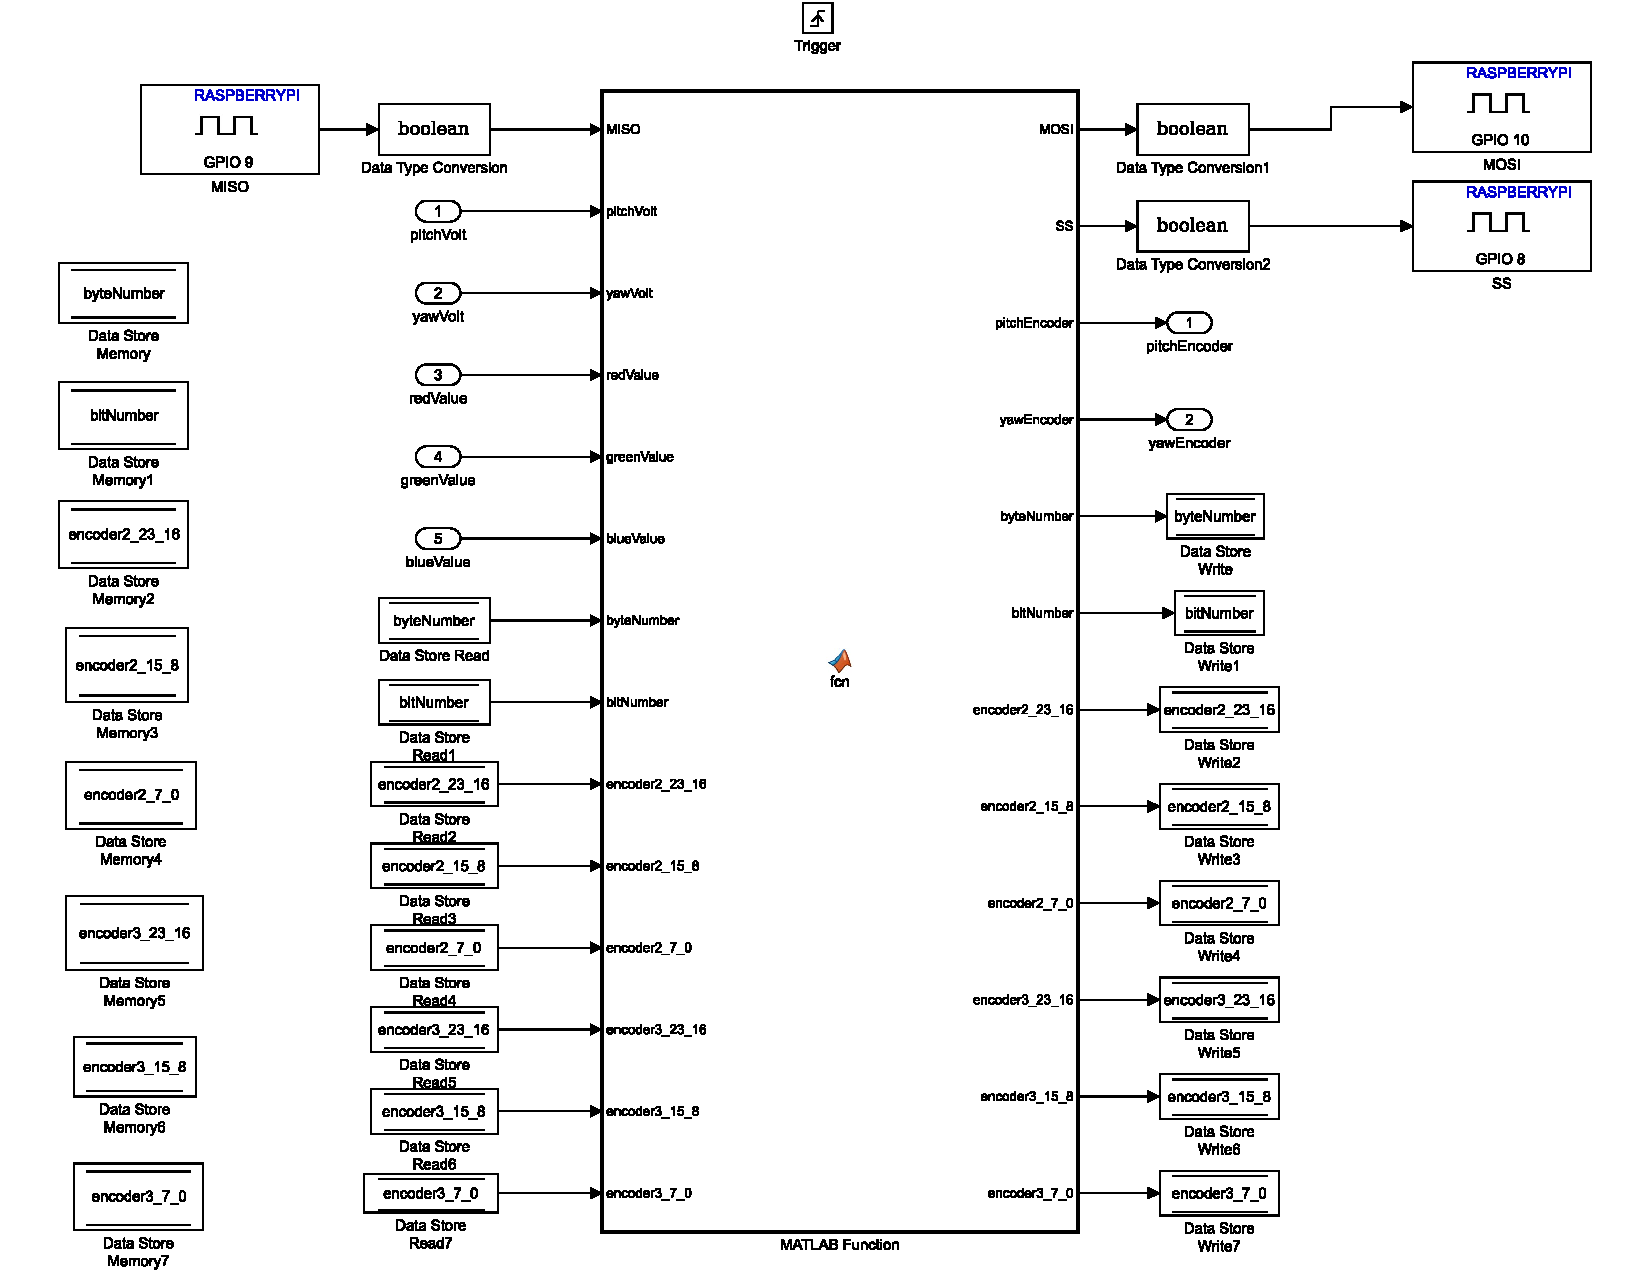
\includegraphics[width=.46\textwidth,keepaspectratio=true]{figs/img/SPI_COM.pdf}
    \label{fig:SPI_COM}
    \caption{Block diagram of SPI communication protocol used for communication between the Raspberry Pi and Quanser Aero.}
\end{figure}


%----------------------------------------------------------------------
\section{Android}
%----------------------------------------------------------------------
\begin{figure}[!htbp]
    \centering
    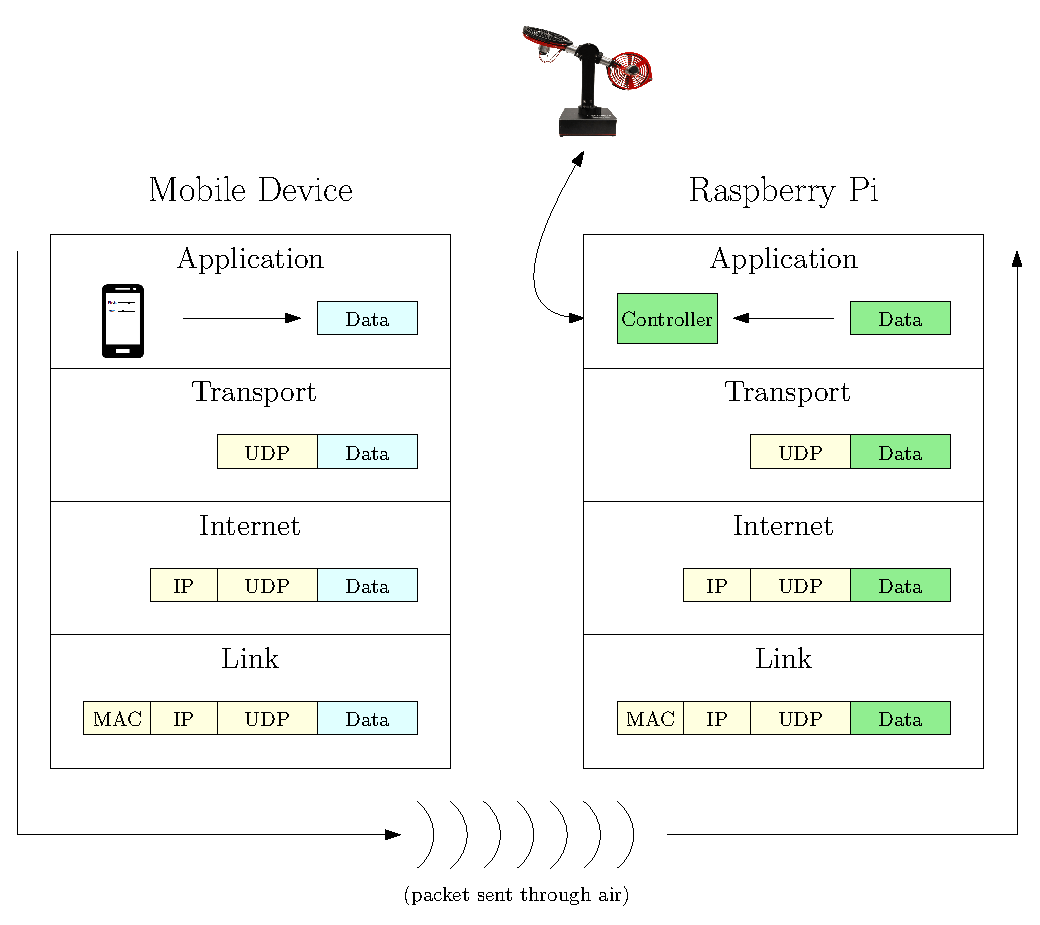
\includegraphics[width=.46\textwidth,keepaspectratio=true]{figs/ipe/TCPModel.eps}
    \label{fig:TCPModel}
    \caption{Illustration of the TCP model which describes how packets are sent and recieved from mobile devices to the Quanser Aero.}
\end{figure}

\begin{figure}[!htbp]
    \centering
    \includegraphics[width=.5\textwidth,keepaspectratio=true]{figs/ipe/Setup.eps}
    \label{fig:Setup}
    \caption{Experiment setup for controlling the Quanser Aeros via a mobile device.}
\end{figure}




%%% Local Variables:
%%% mode: latex
%%% TeX-master: "../finalReportMainV1"
%%% End:
